\documentclass[12pt,a4paper,twoside]{article}

% 1. Paquetes de Idioma y Codificación
\usepackage[utf8]{inputenc}
\usepackage[T1]{fontenc}
\usepackage[spanish, es-tabla]{babel}
\usepackage{tikz}

% 2. Paquetes de Formato y Tablas
\usepackage[utf8]{inputenc}
\usepackage[table,xcdraw]{xcolor} % Para el color gris de las filas
\usepackage{booktabs}             % Para las líneas horizontales (toprule, midrule)
\usepackage{tabularx}
\usepackage{geometry}
\usepackage{tabularx}
\usepackage{booktabs}
\usepackage{array, multirow, multicol}
\usepackage{setspace}
\usepackage{ragged2e}
\usepackage[none]{hyphenat}
\usepackage{enumitem}
\usepackage[table]{xcolor}

% 3. Paquetes Matemáticos y Gráficos
\usepackage{amsmath, amsfonts, amssymb} 
\usepackage{graphicx}
\usepackage{float}
\usepackage{fancyhdr}
% Definimos un tipo de columna 'C' que expande y centra el contenido
\newcolumntype{C}{>{\centering\arraybackslash}X}

% --- Configuración de márgenes TOTALMENTE CORREGIDA ---
\geometry{
	top=4.5cm,      % Espacio para que el texto empiece debajo del banner
	bottom=3cm,
	left=2.5cm,
	right=2.5cm,
	headheight=4cm, % Altura del encabezado
	headsep=0.5cm,
	includehead=false % Importante: false para que TikZ use la hoja completa
}

% ----------------- Configuración de Encabezado -----------------
\pagestyle{fancy}
\fancyhf{} 

\fancyhead[C]{%
	\begin{tikzpicture}[remember picture, overlay]
		% Anclaje al norte absoluto de la página
		\node[anchor=north, inner sep=0pt] at (current page.north) {%
			\includegraphics[width=\paperwidth, height=3.5cm]{Imagenes/ICCU.png}%
		};
	\end{tikzpicture}
}

\renewcommand{\headrulewidth}{0pt} % Sin línea negra

\begin{document}
	
	% Aquí empieza tu contenido

	

	\vspace{0.5cm}
\begin{document}
	% Justificación global
	\justifying 
	\onehalfspacing % Espaciado 1.5 para mejor lectura técnica
	
	% ================= PORTADA =================
	\begin{center}
		
	\subsection*{INSTITUTO DE CAMINOS Y CONSTRUCCIONES DE CUNDINAMARCA}
		
		\bigskip
		\bigskip
		\bigskip
		\bigskip
		\bigskip
		\bigskip
		\bigskip
	
			\bigskip
		\bigskip
		\bigskip
		\bigskip
		
		
		\bigskip
		\bigskip
		\bigskip
		\bigskip
		\bigskip
		\bigskip
		\bigskip
		\bigskip
		
		\subsection*{CONTRATO DE CONSULTORIA No. 259 DE 2025
			“ESTUDIOS Y DISEÑOS PARA LA VÍA DESDE EL SECTOR ESCALANTE HASTA EL CASCO URBANO DEL MUNICIPIO DE TENA VÍA SECTOR SANTA MARTA EN EL MUNICIPIO DE FUSAGASUGÁ”}
		
		\subsection*{VOLUMEN XI. GESTIÓN PREDIAL}
		
		\bigskip
		\bigskip
		\bigskip
		\bigskip
		

		\bigskip
		\bigskip
		\bigskip
		\bigskip
			\bigskip
		\bigskip
		\bigskip
		\bigskip
		
		
		\bigskip
		\bigskip
		\bigskip
		\bigskip

		
		\subsection*{ Febrero del 2026}
		
	\end{center}
\clearpage
% ===========================================

\tableofcontents
\clearpage

% ===== INICIO DEL DOCUMENTO TÉCNICO =====
\justifying

\section{ INTRODUCCIÓN }

El presente documento corresponde al Informe Predial – Tramo 4 Muro Sasaima, elaborado en el marco del CONTRATO DE CONSULTORÍA No. 259 DE 2025, denominado “Estudios y diseños para la vía desde el sector Escalante hasta el casco urbano del municipio de Tena vía sector Santa Marta en el municipio de Fusagasugá”.

En este volumen se presentan los aspectos técnicos analizados y los resultados obtenidos para identificar, evaluar y caracterizar las posibles afectaciones prediales derivadas de los estudios y diseños geométricos, de estructuras y demás componentes asociados al proyecto vial en el tramo objeto de estudio.

El informe tiene como propósito servir de insumo técnico para la gestión predial del proyecto, permitiendo establecer de manera clara las áreas requeridas, los tipos de afectación y las implicaciones sobre los predios involucrados, de conformidad con la normativa vigente y las condiciones particulares del corredor vial analizado.
La información aquí consignada constituye un soporte fundamental para la toma de decisiones durante las etapas de gestión, adquisición y/o intervención predial necesarias para la adecuada ejecución del proyecto.

\subsection{ Objetivo  general }
Determinar e identificar las afectaciones prediales asociadas al proyecto vial, mediante el análisis de la cartografía predial existente y la delimitación de las áreas requeridas para la materialización del trazado definitivo.

\subsection{ Objetivo  específicos }



	\begin{itemize}
	\item Establecer un insumo técnico que apoye los procesos de gestión predial y toma de decisiones del proyecto.
	\item Determinar los predios afectados con base en la cartografía predial existente.
	\item Identificar los inmuebles aledaños al corredor del proyecto que puedan presentar algún tipo de influencia o afectación directa.
	\item Aproximar las áreas afectadas que resultan requeridas para materializar el trazado definitivo y las obras asociadas.
	
\end{itemize}

\section{ Método y alcance }

El presente estudio predial se desarrolla mediante una investigación técnica integral y verificación de los predios, orientada a identificar, delimitar y estimar las áreas afectadas por el proyecto de infraestructura vial correspondiente al tramo cuatro muro Saisaima.
La metodología se fundamenta en la revisión y análisis del ordenamiento territorial vigente, la información catastral disponible y la cartografía base del proyecto, complementada con actividades de campo, con el fin de suministrar a la entidad contratante un inventario organizado, confiable y técnicamente sustentado de los predios involucrados.
Como resultado, se consolida información técnica predial que servirá como insumo para las etapas posteriores de gestión predial, adquisición de áreas, definición de afectaciones y toma de decisiones relacionadas con la ejecución del proyecto, mediante la elaboración de fichas prediales básicas por cada inmueble identificado.

\subsection{ Afectación predial}

El estudio predial y catastral se inicia a partir del trazado conceptual del proyecto vial, el cual constituye la base para la elaboración del Plano General de Afectación Predial. Una vez definidos los diseños geométricos y de estructuras, se procede a estimar el área de afectación de cada una de las zonas de terreno colindantes al trazado proyectado.
A través de este análisis se identifican los predios potencialmente afectados y no afectados, diferenciando las áreas requeridas para la ejecución de las obras, así como las posibles afectaciones temporales o permanentes.
De manera complementaria, mediante investigación directa y visitas de campo, se analizan las características físicas de los predios, tales como los tipos de construcciones existentes, el uso actual del suelo, el destino de los inmuebles y, cuando aplique, la identificación de cultivos y coberturas predominantes en el área de influencia del proyecto.


\subsection{ Elaboración de planos y fichas prediales}
Con base en el plano de afectación predial, se estiman las áreas requeridas para las obras de intervención proyectadas a nivel geométrico, estructural y geotécnico, así como las características físicas y el estado general de los predios involucrados.
Los planos prediales permiten representar gráficamente elementos relevantes como:

	\begin{itemize}
	\item Linderos del predio.
	\item Geometría de los lotes adyacentes.
	\item Infraestructura existente.
	\item Cuerpos de agua y zonas ambientales.
	\item Áreas verdes, árboles, arbustos y demás coberturas.
	\item Construcciones y mejoras (cuando aplique).
	\item Delimitación clara de la zona afectada o zona a adquirir.
\end{itemize}

La ficha predial constituye el documento base del componente predial, en el cual se consolida la información física, catastral y técnica necesaria para el análisis posterior del inmueble. Estas fichas no sustituyen ni constituyen un estudio jurídico de títulos, y se elaboran con base en la información catastral disponible y los resultados del levantamiento técnico realizado.
Cada ficha incluirá, entre otros, datos como:

	\begin{itemize}
	\item Nombre del proyecto.
	 \item Identificación del predio.
	\item Localización.
	\item Área total y área afectada.
	\item Uso del suelo.
\item Observaciones técnicas relevantes para la gestión predial.
	
\end{itemize}

\section{Memoria técnica}

Con base en la información obtenida del levantamiento topográfico ejecutado en campo, se realizó el ajuste y verificación de los linderos de los inmuebles colindantes con el área de intervención del proyecto. Dicho proceso partió de la cartografía catastral oficial del municipio, consultada a través del Gestor Catastral ACC – Agencia Catastral de Cundinamarca, y fue contrastada con la información primaria levantada en sitio.
El ajuste cartográfico se fundamentó en la topografía detallada levantada en campo bajo el sistema de referencia MAGNA–SIRGAS, complementada con la visita técnica preliminar, el análisis de imágenes aéreas captadas mediante dron por el equipo de topografía y la interpretación de imágenes satelitales de apoyo. Esta integración de insumos permitió una delimitación precisa y coherente entre la realidad física del terreno y la información catastral vigente.
De acuerdo con la cartografía ajustada y los análisis espaciales realizados, se establece que las obras proyectadas para el primer tramo —correspondiente a la rehabilitación de muros de contención— se desarrollan íntegramente dentro del corredor existente y no generan afectaciones prediales sobre los inmuebles aledaños. Tal condición se evidencia gráficamente en la Figura 2, donde se observa que las áreas de intervención no sobrepasan los límites de los predios colindantes.
En concordancia con los lineamientos del Manual de Diseño Geométrico de Carreteras del INVIAS, las intervenciones de rehabilitación y estabilización estructural en corredores existentes deben priorizar el aprovechamiento de la franja vial actual, minimizando la adquisición de nuevas áreas y evitando impactos prediales innecesarios, especialmente en tramos con restricciones topográficas y ambientales. Bajo este criterio técnico, el diseño planteado respeta el ancho funcional del corredor y las condiciones geométricas preexistentes, sin requerir ampliaciones laterales que impliquen ocupación de predios privados.
En consecuencia, al no identificarse traslapes, invasiones o afectaciones parciales o totales sobre los bienes inmuebles colindantes, no se contempla la adquisición de áreas ni la imposición de servidumbres para la ejecución del proyecto. Asimismo, dado que no se evidencian conflictos prediales ni interferencias con los linderos legalmente reconocidos, no se considera necesario adelantar análisis detallados de linderos puntuales ni procesos de gestión predial adicional para este tramo del proyecto.

\begin{center}
	% Aumentado a 0.85 para que sea notablemente más grande
	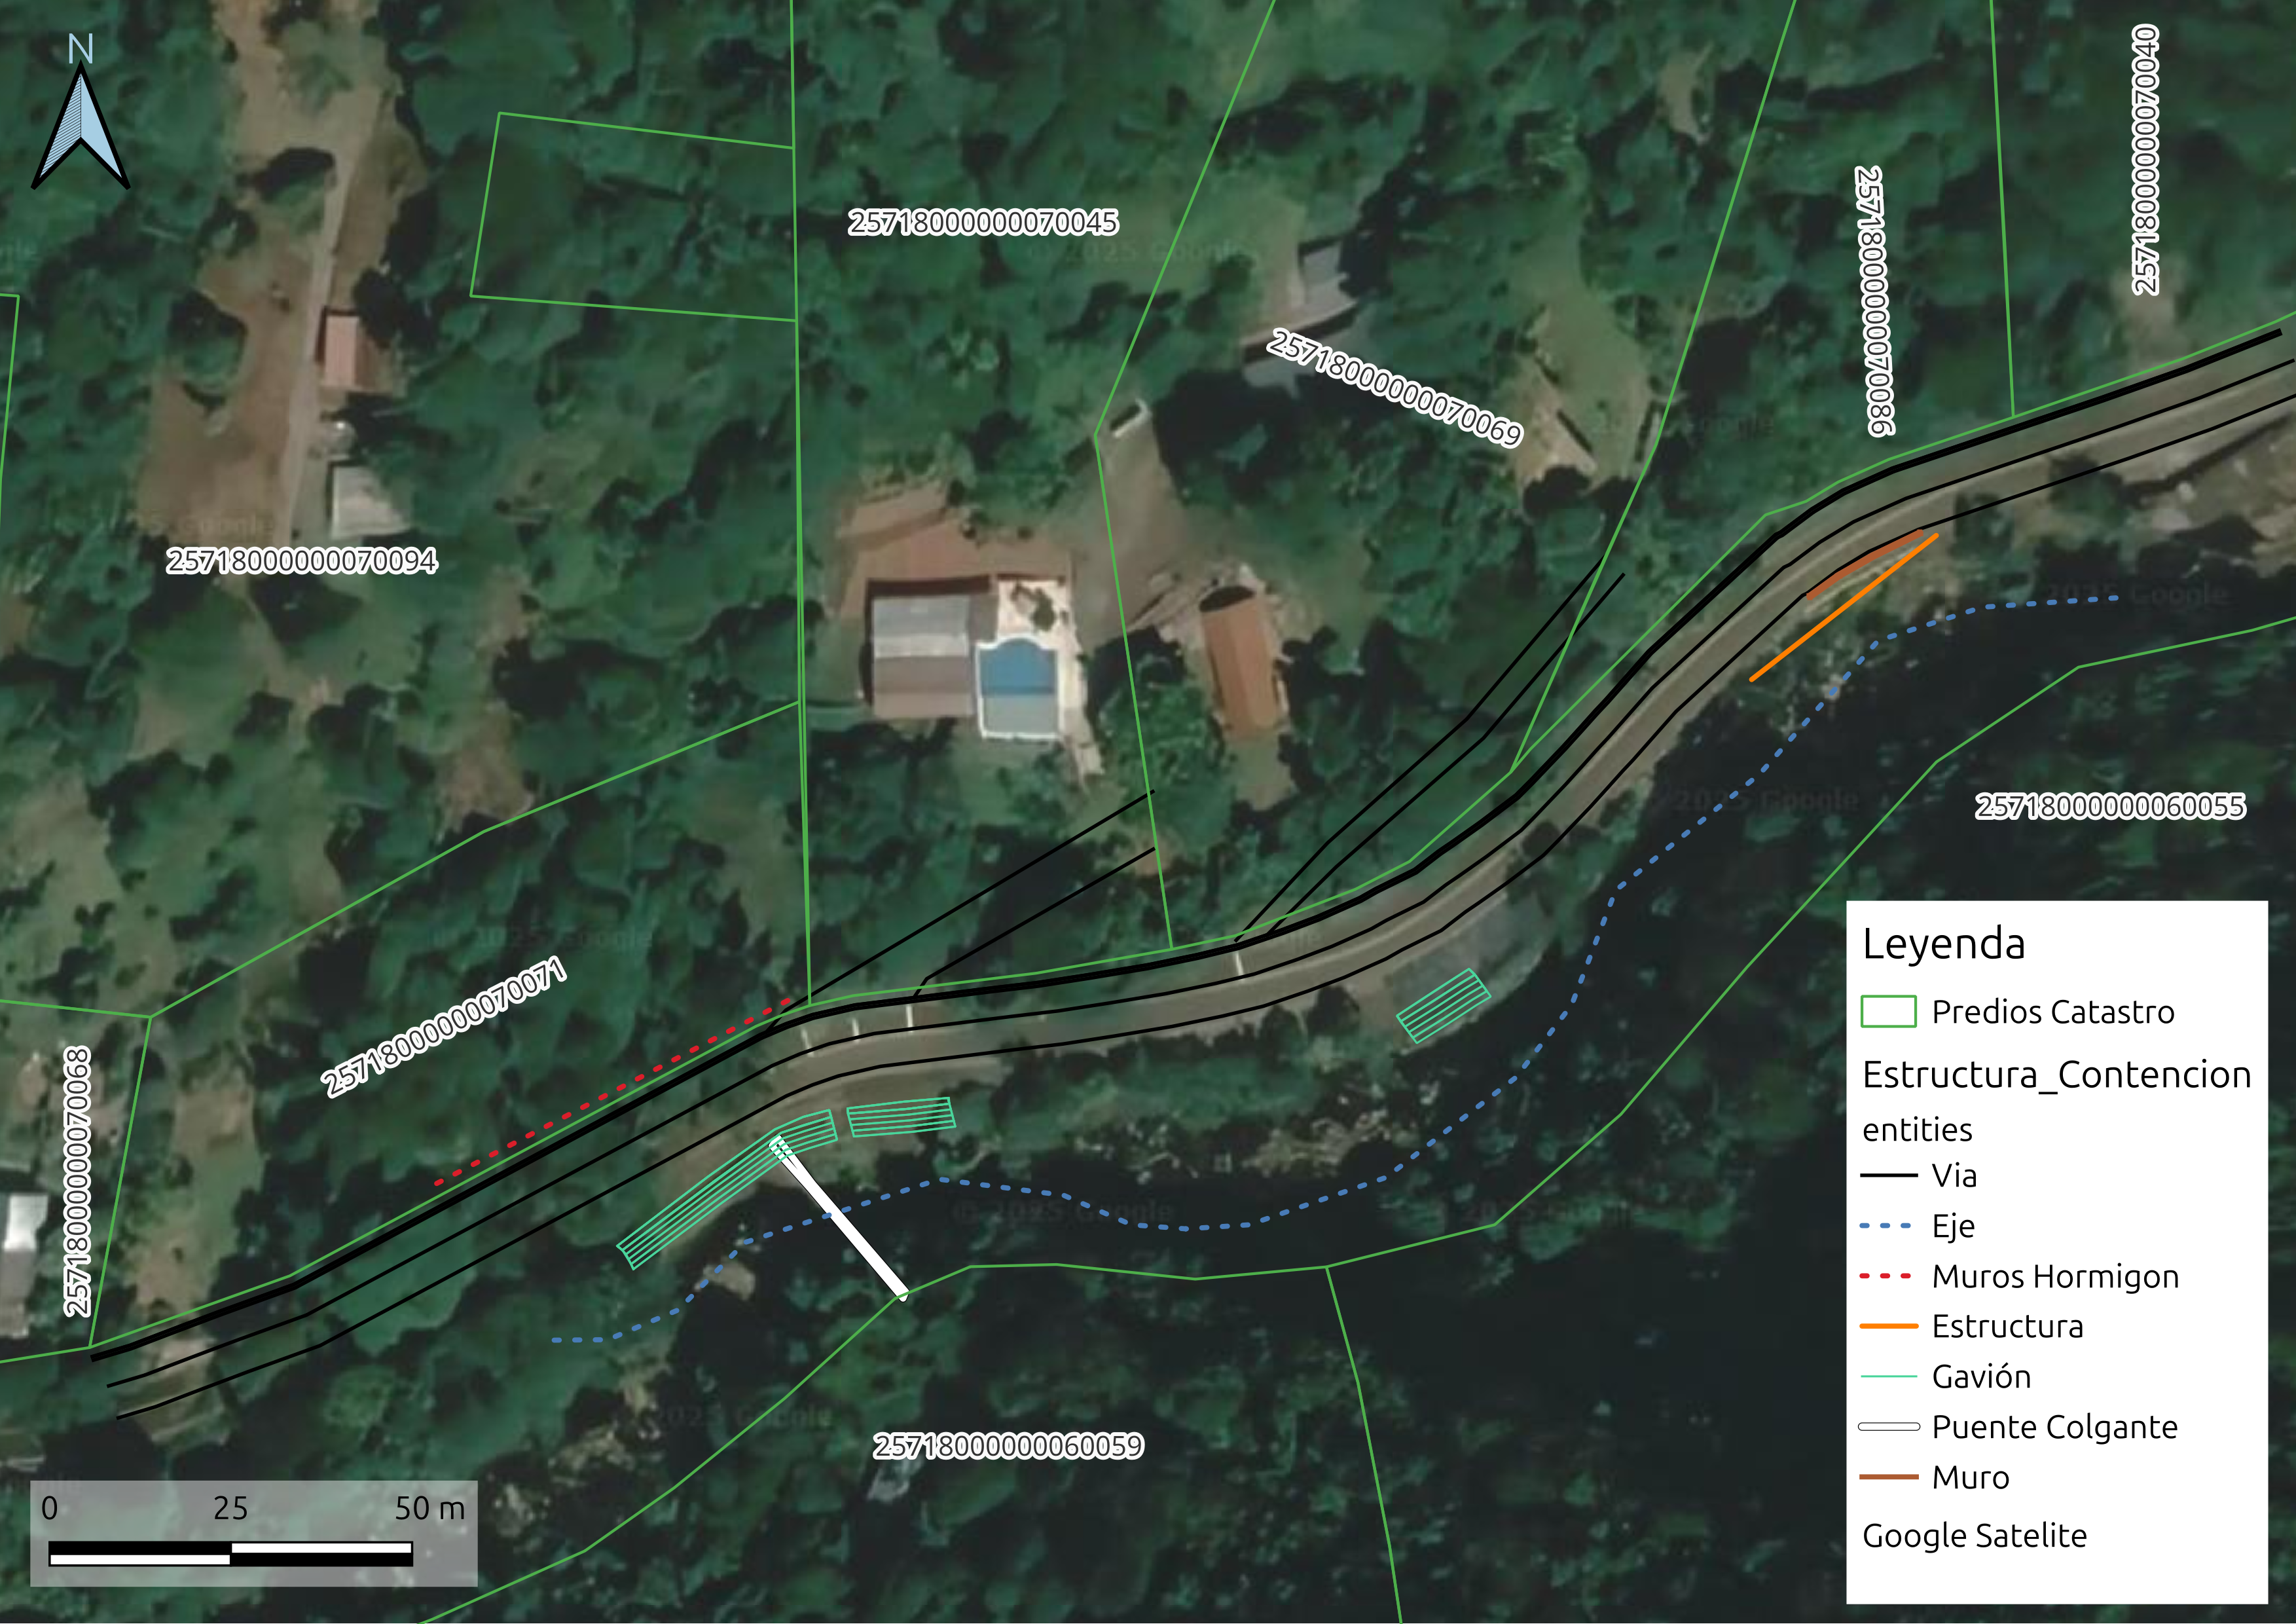
\includegraphics[width=0.85\textwidth]{Imagenes/mapa} 
	\nopagebreak
	
	\vspace{0.2cm} % Añade un pequeño espacio entre imagen y texto
	\small \textbf{Figura 1.} Mapa de predios aledaños.
\end{center}
\vspace{0.2cm}
A continuación se deja una tabla con los códigos prediales y las áreas de cada inmueble, de acuerdo con los cálculos de las mismas, realizadas con el sistema de información geográfica Qgis.

\begin{document}
	
\begin{table}[ht]
	\centering
	\caption{Inmuebles aledaños al proyecto}
	\label{tab:inmuebles}
	% Usamos tabularx para que llegue a los márgenes. 
	% Estructura: c (centrado corto), C (centrado expansivo), c (centrado corto)
	\begin{tabularx}{\textwidth}{c C c}
		\toprule
		\textbf{ID} & \textbf{CODIGO} & \textbf{AREA (m²)} \\ \midrule
		\rowcolor[HTML]{EFEFEF} 
		1           & 25718000000060055 & 65343.06           \\
		2           & 25718000000060059 & 36527.84           \\
		\rowcolor[HTML]{EFEFEF} 
		3           & 25718000000070045 & 27321.39           \\
		4           & 25718000000070068 & 3783.53            \\
		\rowcolor[HTML]{EFEFEF} 
		5           & 25718000000070069 & 16647.13           \\
		6           & 25718000000070094 & 34393.38           \\
		\rowcolor[HTML]{EFEFEF} 
		7           & 25718000000070086 & 3503.35            \\
		8           & 25718000000070071 & 4240.10            \\
		\rowcolor[HTML]{EFEFEF} 
		9           & 25718000000070040 & 259785.77          \\ \bottomrule
	\end{tabularx}
\end{table}
\newpage

\section{Conclusiones}

	\begin{itemize}
	\item La confrontación entre la cartografía catastral oficial y la información levantada en campo permitió validar la correspondencia entre los linderos registrados y la ocupación física en sitio de los predios.
	\item No se identifican traslapes entre el área de intervención del proyecto y los límites de los inmuebles privados, descartando la necesidad de adquisición predial.
	\item La ausencia de afectaciones prediales elimina la necesidad de adelantar procesos de compra de áreas o expropiación.
	\item La información obtenida mediante dron e imágenes satelitales complementó eficazmente el análisis topográfico, fortaleciendo la confiabilidad del ajuste cartográfico.

	
\end{itemize}


\end{document}